\section{Konstrukcja kraty wykładniczej}

W tym podrozdziale omówimy część pracy \cite{10.1145/1007352.1007400}.
Tematem pracy są konstrukcje algorytmów dla problemów $k$-means oraz $k$-median.
W kontekście problemu $k$-means autorzy zaproponowali algorytm rozwiązujący problem $k$-means bazujący na budowie coresetu, który uzyskuje lepszą złożoność od algorytmu przedstawionego w \cite{Matousek99onapproximate}.
Matoušek w swojej pracy \cite{Matousek99onapproximate} przedstawił w pełni wielomianowy schemat aproksymacji, którego złożoność to $O(n\epsilon^{-2k^2d}\log^kn)$.
Autorzy \cite{10.1145/1007352.1007400} poprawili tę złożoność uzyskując $O(n+k^{k+2}\epsilon^{-(2d+1)k}\log^{k+1}n \log^k\frac{1}{\epsilon})$.
Schemat konstrukcji jest następujący:
\begin{itemize}
    \item Obliczmy szybką ale niedokładną aproksymację dla problemu $k$-means z pewną dużą wartością $k$.
    \item Obliczoną aproksymację przekształcamy w $(\epsilon, k)$ coreset używając kraty wykładniczej.
\end{itemize}


\subsection{Szybka aproksymacja dla problemu K-means}
\noindent
Zacznijmy od pierwszej części.
Dokładniej, udowodnimy następujące twierdzenie.

\begin{thm}{\cite{10.1145/1007352.1007400}}
    Dla danego zbioru $n$ punktów $P \subset \mathbb{R}^d$ oraz parametru $k \in \mathbb{N}$ możemy 
    obliczyć zbiór $X$ o mocy $O(k \log^{3}n)$, dla którego 
    \begin{equation}
        \phi_{P}(X) \leq 20 \phi_{opt}^{k}(P)
    \end{equation}
    Czas działania algorytmu to $O(n)$ dla $k = O(n^{\frac{1}{4}})$ oraz $O(n \log (k \log n))$ w przeciwnym przypadku.
\end{thm}

\noindent
Twierdzenie 4.1 w pracy \cite{10.1145/1007352.1007400} ma trochę inną formę.
Ograniczenie jest następujące:
\begin{equation}
    \phi_{P}(X) \leq 32 \phi_{opt}^{k}(P)
\end{equation}
Z analizy, którą zaraz przeprowadzimy wynika, że wspóczynnik aproksymacji jest równy $20$.
Autorzy potrzebowali wspóczynnika równego $32$ z uwagi na inne zastosowanie twierdzenia 4.1 niż nasze.
\\~\\
Niech $P \subset \mathbb{R}^{d}$ będzie danym na wejściu zbiórem $n$ punktów.
Chcemy szybko obliczyć aproksymację dla problemu $k$-means na tym zbiorze, gdzie rozmiar wynikowego zbioru punktów będzie rzędu $O(k \log^{3}n)$.

\begin{definition}
    \emph{Złe/dobre punkty.} Dla zbioru punktów $X$, punkt $p \in P$ nazywamy \textit{złym} jeżeli
    \begin{equation}
        d(p, X) \geq 2d(p, C_{opt})
    \end{equation}
    gdzie $C_{opt}$ jest zbiórem punktów realizującym $\phi_{opt}^{k}(P)$.
    Punkt jest \textit{dobry} jeżeli nie jest zły.
\end{definition}

\noindent
Na początku opiszemy procedurę, która dla danego $P$, wyznacza zbiór punktów $X$ o mocy rzędu $O(k \log^{2}n)$ oraz zbiór $P^{'} \subset P$.
Zbiór $P^{'}$ będzie zawierać \textit{dobre} punkty dla zbioru $X$.
Intuicyjnie procedura ma na celu przekształcenie obliczonej 2-aproksymacji problemu k-centrów dla zbioru $P$ tak, aby rozwiązanie było aplikowalne do problem $k$-means z zachowaniem pewnych gwarancji teoretycznych.
Punkty \textit{dobre} nie wymagają od nas dodatowej pracy, ponieważ dla każego punktu $p \in P^{'}$ instnieje punkt $x \in X$, który \textit{dobrze} aproksymuje wartość $d(p, C_{opt})$, a dokładniej $ d(p, x) \leq 2d(p, C_{opt})$.
\\~\\
Konstrukcję zbioru $X$ zaczynamy od obliczenia 2-aproksymacji problemu k-centrów dla zbioru $P$.
Niech obliczony zbiór centrów to $V$.
Taką aproksymację dla $k = O(n^{\frac{1}{4}})$ możemy obliczyć w czasie $O(n)$ oraz dla $k = \Omega(n^{\frac{1}{4}})$ w czasie $O(n \log k)$ \cite{10.1145/62212.62255}.
Są to wyniki teoretyczne, które zakładamy na potrzebę analizy.
W podrozdziale 4.1 przedstawiliśmy algorytm aproksymacyjny z pracy \cite{Gonzalez1985ClusteringTM}, rozwiązujący ten problem w czasie $O(nk)$ dla dowolnego $k$.
Algorytmy o lepszej złożoności są w istotny sposób bardziej skomplikowane, dlatego w naszej implementacji zastosowaliśmy algorytm Gonzaleza.
Niech $L$ będzie promieniem takiej aproksymacji, czyli największą odległością pomiędzy punktem $v \in V$ a punktem $p \in P-V$, dla którego punkt $v$ jest centrem.
Dla przypomnienia, punkt $v \in V$ będzie centrem dla punktu $p \in P-V$, jeżeli wartość $d(v,p)$ jest najmniejsza spośród wszystkich punktów z $V$.
Ponieważ algorytm z pracy \cite{10.1145/62212.62255} bazuje na algorytmie przedstawionym w podrozdziale 4.1 z pracy \cite{Gonzalez1985ClusteringTM} to dystans pomiędzy dowolną parą punktów z $V$ wynosi co najmniej $L$.
To implikuje następujące ograniczenia:
\begin{equation}
    \Big( \frac{L}{2 } \Big)^2 \leq \phi_{opt}^{k}(V) \leq \phi_{opt}^{k}(P) \leq nL^{2}
\end{equation}
Dolne ograniczenie argumentujemy tym, że możemy ograniczyć $\phi_{opt}^{k}(V)$ przez $d(v_{1}, v_{2})^2$, gdzie $v_{1}, v_{2} \in V$.
Górne ograniczenie wynika z faktu, że promień aproksymacji jest równy $L$, zatem dla $n$ elementowego zbioru $P$ wartość funkcji $\phi_{opt}^{k}(P)$ nie może być większa niż $nL^2$.
\\~\\
Następnym krokiem konstrukcji jest wylosowanie $\rho = \gamma k \log^{2} n$ punktów ze zbioru $P$, gdzie $\gamma$ jest stałą, która wynika z analizy, którą zaraz przeprowadzimy.
Niech $Y$ będzie zbiorem wylosowanych punktów z $P$ oraz $X = Y \cup V$ będzie zbiorem środków klastrów.
Klasterem nazywamy skończony zbioru punktów $x_{1}, \dots, x_{k} \in \mathbb{R}^{d}$, które łączy pewna wspólna cecha.
Dla $\rho > n$ przyjmujemy $X = P$.
\\~\\
Konstrukcja zbioru $X$ jest stosunkowo prosta.
Dużo cięższym zadaniem jest zbudowanie zbioru $P^{'}$, który jest zbiorem \textit{dobrych} punktów dla $X$.

\subsection{Konstrukcja zbioru dobrych punktów dla $X$.}

Rozpatrzmy zbiór $C_{opt}$, który jest optymalnym zbiorem centrów problemu $k$-means dla zbioru $P$ i liczby $k$.
Dla każdego $c_{i} \in C_{opt}$ tworzymy kulę $B_{i}$ o środku w $c_{i}$.
Każda taka kula będzie zawierać co najwyżej $\eta = \frac{n}{20k \log n}$ punktów z $P$.
Jeżeli zastosowana do wylosowania zbioru $X$ stała $\gamma$ jest odpowiednio duża to z wysokim prawdopodobieństwem w każdym $B_{i}$ jest przynajmniej jeden punkt z $X$.
Dokładniej:
\begin{equation}
    X \cap B_{i} \neq \emptyset \text{ dla } i = 1 \dots k
\end{equation}

\noindent
Niech $P_{bad}$ będzie zbiorem złych punktów z $P$ dla zbioru $X$.
Załóżmy, że dla każdego $B_{i}$ istnieje punkt $x_{i} \in X \cap B_{i}$.
Zauważmy, że dla każdego punktu $p \in P \setminus B_{i}$, dla którego $x_{i}$ jest najbliższym punktem z $X$ mamy $||p - x_{i}|| \leq 2||p - c_{i}||$, ponieważ $V \subseteq X$.
W szczególności, jeżeli $c_{i}$ jest najbliższym punktem z $C_{opt}$ dla punktu  $p \in P \setminus B_{i}$, to taki punkt jest \textit{dobry} dla zbioru $X$.
Zatem z wysokim prawdopodobieństwem jedyne \textit{złe} punkty będą w kulach $B_{i}$ dla $ i = 1, \dots, k$.
To implikuje, że z wysokim prawdopodobieństwem liczba złych punktów w $P$ dla zbioru $X$ to co najwyżej $\beta = k\eta = \frac{n}{20 \log n}$.
\\~\\
W takim razie złych punktów nie jest dużo.
Mimo tego bezpośrednie wyznaczenie tych punktów jest skomplikowane.
Autorzy pracy \cite{10.1145/1007352.1007400} budują zbiór $P^{'}$ tak aby koszt złych punktów w $P^{'}$ był jak najmniejszy.
Koszt punktu $p$ w tym kontekście oznacza jaki wkład ma punkt $p$ w wartość $\phi_{P^{'}}(X)$.
Dla każdego punktu w $P$ obliczamy najbliższego sąsiada w $X$.
Niech $r(p) = d(p, X)$ dla każdego punktu $p \in P$.
Teraz podzielimy P na zbiory według następującej formuły:
\begin{equation}
    P[a,b] = \{ p \in P \text{ | } a \leq r(p) \leq b \}
\end{equation}
A dokładniej:
\begin{equation}
    P_{0} = P\Big[0, \frac{L}{4n}\Big]
\end{equation}
\begin{equation}
    P_{ \infty } = P\Big[2Ln, \infty \Big]
\end{equation}
\begin{equation}
    P_{i} = P\Big[ \frac{2^{i-1}L}{n}, \frac{2^{i}L}{n} \Big]
\end{equation}
\\~\\
dla $i = 1, \dots, M$, gdzie $M = 2 \lceil \lg n \rceil + 3$ oraz $L$ to promień aproksymacji.
Taki podział możemy wykonać w czasie linowym.
Niech $P_{\alpha}$ będzię ostatnim zbiorem, który zawiera więcej niż $2\beta = \frac{n}{10 \log n}$ punktów. 
Szukany zbiór zdefiniujemy następująco:
\begin{equation}
    P^{'} = V \cup \bigcup_{i \leq \alpha} P_{i}
\end{equation}
Chcielibyśmy aby $|P^{'}| \geq \frac{n}{2}$ oraz $\phi_{P^{'}}(X) = O(\phi_{P^{'}}(C_{opt}))$.
Teraz udowodnimy, że faktycznie tak zdefiniowane $P^{'}$ spełnia powyższe założenia.

\begin{proof}
    Moc zbioru $P^{'}$ jest na pewno równa conajmniej $\Big(n - |P_{\infty}| - M\frac{n}{10 \log n} \Big)$, gdzie ostatni składni jest mocą wszystkich zbiorów $P_{i}$, które zawierają nie więcej niż $2\beta$ punktów, których jest co najwyżej $M$.
    Zauważmy, że $P_{\infty} \subseteq P_{bad}$ oraz $|P_{bad}| \leq \beta$.
    Zatem:
    \begin{equation}
        |P^{'}| \geq n - \frac{n}{20 \log n} - M \frac{n}{10 \log n}
    \end{equation}
    \begin{equation}
        = n - \Big(\frac{n}{10 \log n}\Big) \Big(M + \frac{1}{2}\Big)
    \end{equation}
    \begin{equation}
        = n - \Big(\frac{n}{10 \log n}\Big) \Big(2 \lceil \lg n \rceil + 3 + \frac{1}{2}\Big)
    \end{equation}
    \begin{equation}
        \geq \frac{n}{2}
    \end{equation}
    Jeżeli $\alpha > 0$, to $|P_{\alpha}| \geq 2\beta = \frac{n}{10 \log n}$.
    Z uwagi na to jak budujemy $P^{'}$ w najgorszym przypadku wszystkie złe punkty będą w $P_{\alpha}$.
    Wtedy takie punkty będą miały największy wpływ na funkcję $\phi$.
    Niech $Q^{'} = P_{\alpha} \setminus P_{bad}$.
    Dla dowolnych punktów $p \in P^{'} \cap P_{bad}$ oraz $q \in Q^{'}$, mamy $d(p, X) \leq 2d(q,X)$, ponieważ $d(p, X) \leq \frac{2^{\alpha}L}{n}$ oraz $d(q, X) \geq \frac{2^{\alpha-1}L}{n}$.
    Dodatkowo $|Q^{'}| > |P_{bad}|$, a więc:
    \begin{equation}
        \phi_{P^{'} \cap P_{bad}}(X) \leq 4\phi_{Q^{'}}(X) \leq 16\phi_{Q^{'}}(C_{opt}) \leq 16\phi_{P^{'}}(C_{opt})
    \end{equation}
    Teraz możemy wyprowadzić następujące ograniczenie:
    \begin{equation}
        \phi_{P^{'}}(X) = \phi_{P^{'} \cap P_{bad}}(X) + \phi_{P^{'} \setminus P_{bad}}(X)
    \end{equation}
    \begin{equation}
        \leq 16\phi_{P^{'}}(C_{opt}) + 4\phi_{P^{'}}(C_{opt}) = 20\phi_{P^{'}}(C_{opt})
    \end{equation}
    Jeżeli $\alpha = 0$, to dla dowolnego punktu $p \in P^{'}$ mamy:
    \begin{equation}
        (d(p,X))^2 \leq n\Big(\frac{L}{4n}\Big)^2 \leq \frac{L^{2}}{16n} \leq \frac{L^{2}}{4n}
    \end{equation}
    Zatem:
    \begin{equation}
        \phi_{P^{'}}(X) \leq \frac{L^{2}}{4} \leq \phi_{V}(C_{opt}) \leq \phi_{P^{'}}(C_{opt})
    \end{equation}
    bo $V \subseteq P^{'}$.
\end{proof}

\noindent
Powyższa analiza dowodzi poprawności konstrukcji dla zbiorów $X$ i $P^{'}$.
Podsumowując otrzymujemy zbiór $X$ o mocy $O(k \log^{2} n)$ oraz zbiór $P^{'}$, dla którego mamy $\phi_{P^{'}}(X) \leq 20\phi_{P^{'}}(C_{opt})$.
Czas działania tego algorytmu to $O(n)$ dla $k = O(n^{\frac{1}{4}})$ oraz $O(n \log (k \log n))$ w przeciwnym przypadku \cite{10.1145/1007352.1007400}.
Aby otrzymać taką złożoność kluczowe jest szybkie obliczenie najbliższych sąsiadów punktów.
Autorzy \cite{10.1145/1007352.1007400} proponują zastosowanie algorytmu przedstawionego w pracy \cite{10.1145/293347.293348}.
\\~\\
Wróćmy teraz do twierdzenia 4.1, które zostało zdefiniowane na początku podrozdziału 4.2.
Chcemy znaleźć zbiór $X^{'}$ o mocy $O(k \log^{3} n)$, dla którego jak najwięcej punktów ze zbióru $P$ jest dobrych.
Powyżej zdefiniowaną procedurę powtarzamy dla zbioru $P_{1} = P \setminus P^{'}$.
Analogicznie otrzymamy zbiór $P_{1}^{'}$ oraz $X_{1}$.
Kolejny raz aplikujemy procedurę na zbiorze $P_{2} = P \setminus (P^{'} \cup P_{1}^{'})$.
Ponieważ za każdym razem zbiór $P_{i}$ zmieniejsza się co najmniej o połowę to taki proces zakończy się po $O(\log n)$ powtórzeniach.
Finalnie otrzymamy zbiór $X^{'} = X \cup X_{1} \dots X_{i}$ o mocy $O(k \log^{3} n)$, dla którego $\phi_{P}(X^{'}) \leq 20\phi_{P}(C_{opt})$.
Złożoność pozostanie taka sama, czyli $O(n)$ dla $k = O(n^{\frac{1}{4}})$ oraz $O(n \log (k \log n))$ w przeciwnym przypadku.

\subsection{Krata wykładnicza.}

Przejdzmy teraz do kluczowej części tego podrozdziału, czyli budowy kraty wykładniczej, która jest autorską konstrukcją \cite{10.1145/1007352.1007400}.
Krata wykładnicza jest obiektem geometrycznym zbudowanym z komórek, które są hipersześcianami.
Każda krata posiada punkt początkowy, od którego zaczynamy konstrukcję przylegających do siebie komórek o zwiększających się długościach boków.
Komórki zawierają punkty z danego na wejścu zbioru danych oraz punkt początkowy jest ustalonym punktem z tego zbioru.
Konstrukcję dzielimy na $\log n$ poziomów, gdzie $n$ jest mocą wejściowego zbioru.
Komórki o tych samych długościach boków należą do tego samego poziomu.
Na rysunku 4.1 widzimy 3 poziomową kartę wykładniczą w $\mathbb{R}^2$.
Komórki są kwadratami a punktem początkowym jest $c$.
\\~\\
Niech $P \subset \mathbb{R}^d$, $|P| = n$ oraz niech $A = \{x_{1}, \dots, x_{m}\}$ będzie zbiorem punktów, dla którego zachodzi $\phi_{P}(A) \leq c\phi_{opt}^{k}(P)$, gdzie $c$ jest stałą.
Nasze $A$ otrzymamy z konstrukcji opisanej w 4.2.1 dla parametru $k = O(k \text{poly} \log n)$ oraz zbioru $P$, gdzie $\text{poly} \log n = \bigcup_{c \geq 1} O(\log^{c}n)$.
Przedstawiony w tym podrozdziale algorytmy oblicza $(k, \epsilon)$-coreset, gdzie $\epsilon \in (0,1)$ oraz $c = 20$.
\\~\\
Niech $R = \sqrt{\frac{\phi_{P}(A)}{cn}}$ będzie dolnym ograniczeniem dla $R_{opt}^{\phi}(P, k) = \sqrt{\frac{\phi_{opt}(P, k)}{n}}$
Niech $P_{i}$ będzie podzbiorem punktów z $P$, dla których punkt $x_{i} \in A$ jest najbliższym sąsiadem. 
Dla dowolnego $p \in P_{i}$, mamy $||px_{i}|| \leq \sqrt{xn}R$, ponieważ $||px_{i}||^{2} \leq \phi_{P}(A)$ dla $i = 1, \dots, m$.
\\~\\
Kolejnym krokiem będzie budowa kraty wykładniczej wokół każdego punktu $x_{i}$.
Niech $Q_{i,j}$ będzie kwatratem o boku długości $R2^{j}$ o środku w punkcie $x_{i}$ dla $j = 0, \dots, M$, gdzie $M = \lceil 2 \lg(cn) \rceil$, który jest równoległy do osi układu współrzednych dla danej przestrzeni.
Następnie, niech $V_{i, 0} = Q_{i, 0}$ oraz niech $V_{i,j} = Q_{i,j} \setminus Q_{i,j-1}$ dla $j = 0, \dots, M$.
Kolejnym krokiem będzie przekształcenie $V_{i,j}$ w kratę, której komórki będą długości $r_{j} = \frac{\epsilon R2^{j}}{10cd}$ oraz niech $G_{i}$ oznacza wynikową kratę wykładniczą dla $V_{i,0}, \dots, V_{i,M}$.
Mając $G_{i}$ obliczamy dla każdego punktu z $P_{i}$ komórkę, do której należy.
Dla każdej niepustej komórki z kraty wybieramy losowy punkt do niej należący, który będzie jej reprezentantem.
Do takiego punktu przypisujemy wagę, która bedzie równa liczbie punktów z komórki, dla której jest reprezentantem.
Po przejściu całej kraty otrzymamy zbiór $S_{i}$ takich punktów.
Definujemy $S = \bigcup_{i} S_{i}$, który jest  $(\epsilon, k)$ coresetem.
Dowód tego, że zbiór $S$ jest $(\epsilon, k)$ coresetem pomijamy z uwagi na jego mechniczność i żmudność.
Można do znaleźć w \cite{10.1145/1007352.1007400}.
Zauważmy, że $|S| = O\Big( \frac{|A| \log n }{ (c\epsilon)^{d} } \Big)$, ponieważ każda krata ma $\log n$ poziomów, a każdy poziom stałą liczbę komórek.
\begin{figure}[H]
    \centering
    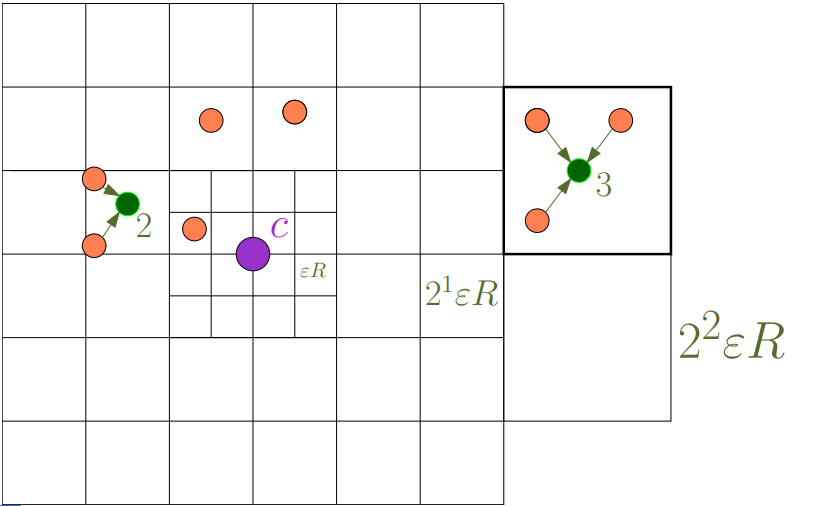
\includegraphics[totalheight=4cm]{grid.png}
    \caption{Krata wykładnicza, gdzie $c = x_{i}$. W najbliższym otoczeniu punktu $c$ widzimy kratę $V_{i,0}$ z długością komórki równej $r_{0} = \epsilon R$.
    Dla uproszczenia pomijam zmienne w mianowniku wcześniej podanej definicji $r_{j}$.
    Kolejny poziom to krata $V_{i,1}$ o długości komórek równej $r_{1} = 2 \epsilon R$.
    Zielone punkty to reprezentanci danej komórki, którym przypisujemy odpowienie wagi równe liczbie punktów w komórce. 
    }
\end{figure}
